\documentclass[border=4pt,12pt]{standalone}
% House style for redrawn exam diagrams (diagram-v4: 0.4pt lines, filled -latex arrows, fine dashes; stipple and hatching drawn as real dots/lines (no PDF/SVG patterns, so they render in every browser and at any scale); transparent background). Every figure \input's this.
\usepackage{amsmath,amssymb}
\usepackage{txfonts}
\usepackage{pdfrender,xcolor}
% \halo{text}: label on shading. The shading stops just around each letter's outline (a thin knock-out that follows the
% glyphs, like the papers' typesetting), never a box. Owner: "I don't want a box around the text".
\newcommand{\halo}[1]{\leavevmode\rlap{\pdfrender{TextRenderingMode=2,LineWidth=2.2pt,LineJoinStyle=1,StrokeColor=white,FillColor=white}#1}#1}
\usepackage{tikz,pgfplots}
\pgfplotsset{compat=1.18}
\usetikzlibrary{arrows.meta,calc,angles,quotes,patterns,patterns.meta,intersections,positioning,decorations.markings,shapes.geometric}
% Stipple and hatching are drawn as actual dots / lines clipped to the region (path picture), NOT as pattern fills:
% SVG <pattern> fills vanish or blur when browsers scale the image, so the owner could not see the shading.
% Each dot is a 0.72pt square (keeps SVGs small; reads as a dot at print size). Dots sit on one global staggered grid, so neighbouring regions line up.
\makeatletter
\newdimen\ex@x \newdimen\ex@y \newdimen\ex@xa \newdimen\ex@ya \newdimen\ex@xb \newdimen\ex@yb \newcount\ex@row
\def\exam@stipplecolor{black!75}\def\exam@dotr{0.42pt}\def\exam@dotgap{2.5}
\def\ex@rowdots{\ifdim\ex@x<\ex@xb \pgfpathrectangle{\pgfqpoint{\dimexpr\ex@x-0.36pt\relax}{\dimexpr\ex@y-0.36pt\relax}}{\pgfqpoint{0.72pt}{0.72pt}}\advance\ex@x by \exam@dotgap pt\relax\expandafter\ex@rowdots\fi}
\def\exam@stipple{%
  \pgftransformreset% dots are sized in real points even inside scaled pictures
  \pgfpointanchor{path picture bounding box}{south west}\ex@xa=\pgf@x \ex@ya=\pgf@y
  \pgfpointanchor{path picture bounding box}{north east}\ex@xb=\pgf@x \ex@yb=\pgf@y
  \pgfsetfillcolor{\exam@stipplecolor}\pgfmathsetmacro\ex@h{\exam@dotgap/2}%
  \pgfmathtruncatemacro\ex@r{floor(\ex@ya/\ex@h)-1}\ex@row=\ex@r\relax
  \ex@y=\ex@r\dimexpr\ex@h pt\relax
  \loop\ifdim\ex@y<\ex@yb
    \pgfmathtruncatemacro\ex@c{floor(\ex@xa/\exam@dotgap)-1}\ex@x=\ex@c\dimexpr\exam@dotgap pt\relax
    \ifodd\ex@row \advance\ex@x by \ex@h pt\fi
    \ex@rowdots
    \advance\ex@y by \ex@h pt \advance\ex@row by 1
    \ifnum\numexpr\ex@row-(\ex@row/4)*4\relax=0 \pgfusepath{fill}\fi% flush every 4 rows: bounded TeX memory, few clip copies in the SVG
  \repeat\pgfusepath{fill}}
\newdimen\ex@d
\def\exam@hatch#1{% #1 = 1 for /, -1 for \ ; lines 45 degrees, 3pt apart
  \pgftransformreset
  \pgfpointanchor{path picture bounding box}{south west}\ex@xa=\pgf@x \ex@ya=\pgf@y
  \pgfpointanchor{path picture bounding box}{north east}\ex@xb=\pgf@x \ex@yb=\pgf@y
  \ex@d=\dimexpr\ex@yb-\ex@ya\relax \ex@x=\dimexpr\ex@xa-\ex@d\relax
  \loop\ifdim\ex@x<\ex@xb
    \ifnum#1>0 \pgfpathmoveto{\pgfqpoint{\ex@x}{\ex@ya}}\pgfpathlineto{\pgfqpoint{\dimexpr\ex@x+\ex@d\relax}{\ex@yb}}%
    \else \pgfpathmoveto{\pgfqpoint{\ex@x}{\ex@yb}}\pgfpathlineto{\pgfqpoint{\dimexpr\ex@x+\ex@d\relax}{\ex@ya}}\fi
    \advance\ex@x by 4.24pt
  \repeat
  \pgfsetlinewidth{0.4pt}\pgfsetstrokecolor{black}\pgfusepath{stroke}}
\def\examstipple{\exam@stipple}\def\examhatch{\exam@hatch}\def\examsetstipplecolor#1{\def\exam@stipplecolor{#1}}\def\examsetdotgap#1{\def\exam@dotgap{#1}}
\makeatother
% (legacy pattern kept for old files)
% staggered stipple like the NESA papers' dotted shading
\pgfdeclarepatternformonly{exam stipple}{\pgfpointorigin}{\pgfqpoint{2.2pt}{2.2pt}}{\pgfqpoint{2.2pt}{2.2pt}}{%
  \pgfpathcircle{\pgfqpoint{0.55pt}{0.55pt}}{0.42pt}\pgfpathcircle{\pgfqpoint{1.65pt}{1.65pt}}{0.42pt}\pgfusepath{fill}}
\tikzset{
  every picture/.style={line width=0.6pt, >={Latex[length=2mm,width=1.3mm]}},
  curve/.style={line width=0.6pt},
  open arrow/.style={-{Latex[length=2mm,width=1.3mm]}},  % owner: filled -latex heads everywhere, no open chevrons
  aux/.style={dash pattern=on 2pt off 1.5pt, line width=0.6pt},
  shade/.code={\def\exA{#1}\def\exB{none}\ifx\exA\exB\else\pgfkeysalso{fill=black!18}\fi},
  shade/.default=on,
  shade dots/.style={fill=none, path picture={\examstipple}},
  stipple color/.code={\examsetstipplecolor{#1}},
  stipple gap/.code={\examsetdotgap{#1}},
  shade dense dots/.style={fill=none, stipple gap=1.6, path picture={\examstipple}},
  shade hatch/.style={fill=none, path picture={\examhatch{1}}},
  shade hatch reverse/.style={fill=none, path picture={\examhatch{-1}}},
  shade solid/.style={fill=black},
  pt/.style={circle, fill, inner sep=1.1pt},
  open pt/.style={circle, draw, fill=white, inner sep=1.1pt},
}
\pgfplotsset{
  exam axes/.style={axis lines=middle, axis line style={->}, xlabel={$x$}, ylabel={$y$},
    xlabel style={anchor=west}, ylabel style={anchor=south}, tick label style={font=\small},
    every axis plot/.append style={line width=0.6pt, black}, samples=200, clip=false,
    enlargelimits=false, axis on top},
}

\begin{document}
% clean redraw of the marking-guideline sketch on its grid (crop pixel units, y down):
% origin (306.5,290.5), 28.95 px per x unit, 34.0 px per y unit (grid cells are not square in the crop).
% Line y=x-2 exact. Cubic follows the sketch (min ~-8.2 near x=0.2, right branch reaching the arrow at (3,4.2)) as a smooth
% curve through points read from the crop, pinned to the labelled (-3,-5),(-2,0),(-1,-3),(0,-8),(2,0); marker notes omitted.
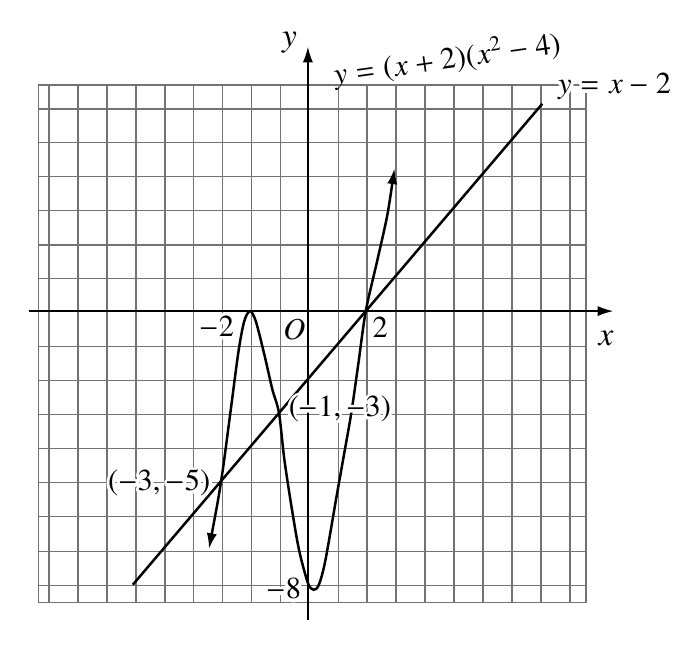
\begin{tikzpicture}[x=0.0127cm,y=-0.0127cm, every node/.style={inner sep=0pt, font=\fontsize{11}{13}\selectfont}]
  \def\X#1{306.5+28.95*(#1)}\def\Y#1{290.5-34.0*(#1)}
  \begin{scope}[black!55]
    \draw (37,64) rectangle (585,582);
    \foreach \x in {47.5,76.5,105.4,134.3,163.3,192.2,221.2,250.2,279.1,337.0,365.9,394.9,423.8,452.8,481.8,510.7,539.6,568.6} \draw (\x,64) -- (\x,582);
    \foreach \y in {88,122,156,190,224.5,258,326,360,394,428,462,496,531,565} \draw (37,\y) -- (585,\y);
  \end{scope}
  \draw[->] (27,290.5) -- (612,290.5);
  \draw[->] (306.5,600) -- (306.5,26);
  \node[font=\fontsize{12}{14}\selectfont] at (604,318) {$x$};
  \node[font=\fontsize{12}{14}\selectfont] at (288,22) {$y$};
  \node at (293,309) {$O$};
  \draw[<->,line width=0.9pt] plot[smooth] coordinates {(207.5,528.5) (219.7,460.5) (228.9,392.5) (237.0,331.3) (242.8,300.7) (248.6,290.5) (254.4,300.7) (263.1,334.7) (270.9,368.7) (277.6,392.5) (283.1,440.1) (290.9,491.1) (297.8,530.2) (306.5,562.5) (312.3,569.3) (317.5,564.2) (323.9,540.4) (334.9,477.5) (343.0,431.9) (349.9,392.5) (357.2,341.5) (364.4,290.5) (376.0,239.5) (386.1,193.6) (393.1,147.7)};
  \draw[line width=0.9pt] plot[domain=-6.05:8.1] ({\X{\x}},{\Y{\x-2}});
  \node[anchor=north east] at ({\X{-2}-15},{\Y{0}+4}) {\halo{$-2$}};
  \node[anchor=north west] at ({\X{2}+6},{\Y{0}+5}) {\halo{$2$}};
  \node[anchor=east] at ({\X{0}-6},{\Y{-8}+6}) {\halo{$-8$}};
  \node[anchor=east] at ({\X{-3}-10},{\Y{-5}+2}) {\halo{$(-3,-5)$}};
  \node[anchor=west] at ({\X{-1}+9},{\Y{-3}-4}) {\halo{$(-1,-3)$}};
  \node[anchor=south, rotate=8] at (448,55) {$y=(x+2)(x^2-4)$};
  \node[anchor=west] at (556,66) {\halo{$y=x-2$}};
\end{tikzpicture}
\end{document}
